
%-----------------------------------------------------------------------------
% PACKAGES AND OTHER DOCUMENT CONFIGURATIONS
%-----------------------------------------------------------------------------

\documentclass[11pt]{article}
\usepackage[margin=1in]{geometry}
\usepackage{amsmath, amsfonts}
\usepackage{enumerate}
\usepackage{graphicx}
\usepackage{titling}
\usepackage{url}
\usepackage{xfrac}
\usepackage{fancyhdr}
\usepackage{geometry}
\usepackage{graphicx}
\usepackage{natbib}
\usepackage{amsmath}
\usepackage{amssymb}
\usepackage{amsthm}
\usepackage{paralist}
\usepackage{epstopdf}
\usepackage{tabularx}
\usepackage{longtable}
\usepackage{minted}
\usemintedstyle{borland}
\usepackage{multirow}
\usepackage{multicol}
\usepackage[colorlinks=true,urlcolor=blue]{hyperref}
\usepackage{fancyvrb}
\usepackage{algorithm}
\usepackage{algorithmicx}
\usepackage[noend]{algpseudocode}
\usepackage{float}
\usepackage{paralist}
\usepackage[svgname]{xcolor}
\usepackage{enumerate}
\usepackage{array}
\usepackage{times}
\usepackage{url}
\usepackage{fancyhdr}
\usepackage{comment}
\usepackage{environ}
\usepackage{times}
\usepackage{textcomp}
\usepackage{caption}
\usepackage[colorlinks=true,urlcolor=blue]{hyperref}
\usepackage{parskip} % For NIPS style paragraphs.
\usepackage[compact]{titlesec} % Less whitespace around titles
\usepackage[inline]{enumitem} % For inline enumerate* and itemize*
\usepackage{datetime}
\usepackage{comment}
% \usepackage{minted}
\usepackage{lastpage}
\usepackage{color}
\usepackage{xcolor}
\usepackage[final]{listings}
\usepackage{tikz}
\usetikzlibrary{shapes,decorations}
\usepackage{framed}
\usepackage{booktabs}
\usepackage{cprotect}
\usepackage{fancyvrb}
\usepackage{xcolor}
\usepackage{verbatimbox}
\usepackage{multicol}
\usepackage{hyperref}
\usepackage{subcaption}
\usepackage{mathtools} % For drcases
\usepackage{cancel}
\usepackage[many]{tcolorbox}
\usepackage{multicol}
\usepackage{sectsty}
\usepackage{bm}
\usepackage{nicefrac}

%%%%%%%%%%%%%%%%%%%%%%%%%%%%%%%%%%%%%%%%%%%
% Better numbering                        %
%%%%%%%%%%%%%%%%%%%%%%%%%%%%%%%%%%%%%%%%%%%

\numberwithin{equation}{section} % Number equations within sections (i.e. 1.1, 1.2, 2.1, 2.2 instead of 1, 2, 3, 4)
\numberwithin{figure}{section} % Number figures within sections (i.e. 1.1, 1.2, 2.1, 2.2 instead of 1, 2, 3, 4)
\numberwithin{table}{section} % Number tables within sections (i.e. 1.1, 1.2, 2.1, 2.2 instead of 1, 2, 3, 4)

%%%%%%%%%%%%%%%%%%%%%%%%%%%%%%%%%%%%%%%%%%
% Custom commands                        %
%%%%%%%%%%%%%%%%%%%%%%%%%%%%%%%%%%%%%%%%%%
\newcommand{\blackcircle}{\tikz\draw[black,fill=black] (0,0) circle (1ex);}
\renewcommand{\circle}{\tikz\draw[black] (0,0) circle (1ex);}
\newcommand{\vc}[1]{\boldsymbol{#1}}
\newcommand{\adj}[1]{\frac{d J}{d #1}}
\newcommand{\chain}[2]{\adj{#2} = \adj{#1}\frac{d #1}{d #2}}
\newcommand{\ntset}{test}
\DeclareMathOperator{\Median}{Median}

% mathcal
\newcommand{\Ac}{\mathcal{A}}
\newcommand{\Bc}{\mathcal{B}}
\newcommand{\Cc}{\mathcal{C}}
\newcommand{\Dc}{\mathcal{D}}
\newcommand{\Ec}{\mathcal{E}}
\newcommand{\Fc}{\mathcal{F}}
\newcommand{\Gc}{\mathcal{G}}
\newcommand{\Hc}{\mathcal{H}}
\newcommand{\Ic}{\mathcal{I}}
\newcommand{\Jc}{\mathcal{J}}
\newcommand{\Kc}{\mathcal{K}}
\newcommand{\Lc}{\mathcal{L}}
\newcommand{\Mc}{\mathcal{M}}
\newcommand{\Nc}{\mathcal{N}}
\newcommand{\Oc}{\mathcal{O}}
\newcommand{\Pc}{\mathcal{P}}
\newcommand{\Qc}{\mathcal{Q}}
\newcommand{\Rc}{\mathcal{R}}
\newcommand{\Sc}{\mathcal{S}}
\newcommand{\Tc}{\mathcal{T}}
\newcommand{\Uc}{\mathcal{U}}
\newcommand{\Vc}{\mathcal{V}}
\newcommand{\Wc}{\mathcal{W}}
\newcommand{\Xc}{\mathcal{X}}
\newcommand{\Yc}{\mathcal{Y}}
\newcommand{\Zc}{\mathcal{Z}}

% mathbb
\newcommand{\Ab}{\mathbb{A}}
\newcommand{\Bb}{\mathbb{B}}
\newcommand{\Cb}{\mathbb{C}}
\newcommand{\Db}{\mathbb{D}}
\newcommand{\Eb}{\mathbb{E}}
\newcommand{\Fb}{\mathbb{F}}
\newcommand{\Gb}{\mathbb{G}}
\newcommand{\Hb}{\mathbb{H}}
\newcommand{\Ib}{\mathbb{I}}
\newcommand{\Jb}{\mathbb{J}}
\newcommand{\Kb}{\mathbb{K}}
\newcommand{\Lb}{\mathbb{L}}
\newcommand{\Mb}{\mathbb{M}}
\newcommand{\Nb}{\mathbb{N}}
\newcommand{\Ob}{\mathbb{O}}
\newcommand{\Pb}{\mathbb{P}}
\newcommand{\Qb}{\mathbb{Q}}
\newcommand{\Rb}{\mathbb{R}}
\newcommand{\Sb}{\mathbb{S}}
\newcommand{\Tb}{\mathbb{T}}
\newcommand{\Ub}{\mathbb{U}}
\newcommand{\Vb}{\mathbb{V}}
\newcommand{\Wb}{\mathbb{W}}
\newcommand{\Xb}{\mathbb{X}}
\newcommand{\Yb}{\mathbb{Y}}
\newcommand{\Zb}{\mathbb{Z}}

% mathbf lowercase
\newcommand{\av}{\mathbf{a}}
\newcommand{\bv}{\mathbf{b}}
\newcommand{\cv}{\mathbf{c}}
\newcommand{\dv}{\mathbf{d}}
\newcommand{\ev}{\mathbf{e}}
\newcommand{\fv}{\mathbf{f}}
\newcommand{\gv}{\mathbf{g}}
\newcommand{\hv}{\mathbf{h}}
\newcommand{\iv}{\mathbf{i}}
\newcommand{\jv}{\mathbf{j}}
\newcommand{\kv}{\mathbf{k}}
\newcommand{\lv}{\mathbf{l}}
\newcommand{\mv}{\mathbf{m}}
\newcommand{\nv}{\mathbf{n}}
\newcommand{\ov}{\mathbf{o}}
\newcommand{\pv}{\mathbf{p}}
\newcommand{\qv}{\mathbf{q}}
\newcommand{\rv}{\mathbf{r}}
\newcommand{\sv}{\mathbf{s}}
\newcommand{\tv}{\mathbf{t}}
\newcommand{\uv}{\mathbf{u}}
\newcommand{\vv}{\mathbf{v}}
\newcommand{\wv}{\mathbf{w}}
\newcommand{\xv}{\mathbf{x}}
\newcommand{\yv}{\mathbf{y}}
\newcommand{\zv}{\mathbf{z}}

% mathbf uppercase
\newcommand{\Av}{\mathbf{A}}
\newcommand{\Bv}{\mathbf{B}}
\newcommand{\Cv}{\mathbf{C}}
\newcommand{\Dv}{\mathbf{D}}
\newcommand{\Ev}{\mathbf{E}}
\newcommand{\Fv}{\mathbf{F}}
\newcommand{\Gv}{\mathbf{G}}
\newcommand{\Hv}{\mathbf{H}}
\newcommand{\Iv}{\mathbf{I}}
\newcommand{\Jv}{\mathbf{J}}
\newcommand{\Kv}{\mathbf{K}}
\newcommand{\Lv}{\mathbf{L}}
\newcommand{\Mv}{\mathbf{M}}
\newcommand{\Nv}{\mathbf{N}}
\newcommand{\Ov}{\mathbf{O}}
\newcommand{\Pv}{\mathbf{P}}
\newcommand{\Qv}{\mathbf{Q}}
\newcommand{\Rv}{\mathbf{R}}
\newcommand{\Sv}{\mathbf{S}}
\newcommand{\Tv}{\mathbf{T}}
\newcommand{\Uv}{\mathbf{U}}
\newcommand{\Vv}{\mathbf{V}}
\newcommand{\Wv}{\mathbf{W}}
\newcommand{\Xv}{\mathbf{X}}
\newcommand{\Yv}{\mathbf{Y}}
\newcommand{\Zv}{\mathbf{Z}}

% bold greek lowercase
\newcommand{\alphav     }{\boldsymbol \alpha     }
\newcommand{\betav      }{\boldsymbol \beta      }
\newcommand{\gammav     }{\boldsymbol \gamma     }
\newcommand{\deltav     }{\boldsymbol \delta     }
\newcommand{\epsilonv   }{\boldsymbol \epsilon   }
\newcommand{\varepsilonv}{\boldsymbol \varepsilon}
\newcommand{\zetav      }{\boldsymbol \zeta      }
\newcommand{\etav       }{\boldsymbol \eta       }
\newcommand{\thetav     }{\boldsymbol \theta     }
\newcommand{\varthetav  }{\boldsymbol \vartheta  }
\newcommand{\iotav      }{\boldsymbol \iota      }
\newcommand{\kappav     }{\boldsymbol \kappa     }
\newcommand{\varkappav  }{\boldsymbol \varkappa  }
\newcommand{\lambdav    }{\boldsymbol \lambda    }
\newcommand{\muv        }{\boldsymbol \mu        }
\newcommand{\nuv        }{\boldsymbol \nu        }
\newcommand{\xiv        }{\boldsymbol \xi        }
\newcommand{\omicronv   }{\boldsymbol \omicron   }
\newcommand{\piv        }{\boldsymbol \pi        }
\newcommand{\varpiv     }{\boldsymbol \varpi     }
\newcommand{\rhov       }{\boldsymbol \rho       }
\newcommand{\varrhov    }{\boldsymbol \varrho    }
\newcommand{\sigmav     }{\boldsymbol \sigma     }
\newcommand{\varsigmav  }{\boldsymbol \varsigma  }
\newcommand{\tauv       }{\boldsymbol \tau       }
\newcommand{\upsilonv   }{\boldsymbol \upsilon   }
\newcommand{\phiv       }{\boldsymbol \phi       }
\newcommand{\varphiv    }{\boldsymbol \varphi    }
\newcommand{\chiv       }{\boldsymbol \chi       }
\newcommand{\psiv       }{\boldsymbol \psi       }
\newcommand{\omegav     }{\boldsymbol \omega     }

% bold greek uppercase
\newcommand{\Gammav     }{\boldsymbol \Gamma     }
\newcommand{\Deltav     }{\boldsymbol \Delta     }
\newcommand{\Thetav     }{\boldsymbol \Theta     }
\newcommand{\Lambdav    }{\boldsymbol \Lambda    }
\newcommand{\Xiv        }{\boldsymbol \Xi        }
\newcommand{\Piv        }{\boldsymbol \Pi        }
\newcommand{\Sigmav     }{\boldsymbol \Sigma     }
\newcommand{\Upsilonv   }{\boldsymbol \Upsilon   }
\newcommand{\Phiv       }{\boldsymbol \Phi       }
\newcommand{\Psiv       }{\boldsymbol \Psi       }
\newcommand{\Omegav     }{\boldsymbol \Omega     }

% Macros
\usepackage{xspace}
\makeatletter
\DeclareRobustCommand\onedot{\futurelet\@let@token\@onedot}
\def\@onedot{\ifx\@let@token.\else.\null\fi\xspace}

\def\eg{\emph{e.g}\onedot} \def\Eg{\emph{E.g}\onedot}
\def\ie{\emph{i.e}\onedot} \def\Ie{\emph{I.e}\onedot}
\def\cf{\emph{c.f}\onedot} \def\Cf{\emph{C.f}\onedot}
\def\etc{\emph{etc}\onedot} \def\vs{\emph{vs}\onedot}
\def\wrt{w.r.t\onedot} \def\dof{d.o.f\onedot}
\def\etal{\emph{et al}\onedot}
\makeatother

% \DeclareFontFamily{\encodingdefault}{\ttdefault}{\hyphenchar\font=`\-}

%%%%%%%%%%%%%%%%%%%%%%%%%%%%%%%%%%%%%%%%%%%
% Code highlighting with listings         %
%%%%%%%%%%%%%%%%%%%%%%%%%%%%%%%%%%%%%%%%%%%

\definecolor{bluekeywords}{rgb}{0.13,0.13,1}
\definecolor{greencomments}{rgb}{0,0.5,0}
\definecolor{redstrings}{rgb}{0.9,0,0}
\definecolor{light-gray}{gray}{0.95}

\newcommand{\MYhref}[3][blue]{\href{#2}{\color{#1}{#3}}}%

\definecolor{dkgreen}{rgb}{0,0.6,0}
\definecolor{gray}{rgb}{0.5,0.5,0.5}
\definecolor{mauve}{rgb}{0.58,0,0.82}

\lstdefinelanguage{Shell}{
  keywords={tar, cd, make},
  %keywordstyle=\color{bluekeywords}\bfseries,
  alsoletter={+},
  ndkeywords={python, py, javac, java, gcc, c, g++, cpp, .txt, octave, m, .tar},
  %ndkeywordstyle=\color{bluekeywords}\bfseries,
  identifierstyle=\color{black},
  sensitive=false,
  comment=[l]{//},
  morecomment=[s]{/*}{*/},
  commentstyle=\color{purple}\ttfamily,
  %stringstyle=\color{red}\ttfamily,
  morestring=[b]',
  morestring=[b]",
  backgroundcolor = \color{light-gray}
}

\lstset{columns=fixed, basicstyle=\ttfamily,
    backgroundcolor=\color{light-gray},xleftmargin=0.5cm,frame=tlbr,framesep=4pt,framerule=0pt}


%%%%%%%%%%%%%%%%%%%%%%%%%%%%%%%%%%%%%%%%%%%
% Custom box for highlights               %
%%%%%%%%%%%%%%%%%%%%%%%%%%%%%%%%%%%%%%%%%%%

% Define box and box title style
\tikzstyle{mybox} = [fill=blue!10, very thick,
    rectangle, rounded corners, inner sep=1em, inner ysep=1em]

% \newcommand{\notebox}[1]{
% \begin{tikzpicture}
% \node [mybox] (box){%
%     \begin{minipage}{\textwidth}
%     #1
%     \end{minipage}
% };
% \end{tikzpicture}%
% }

\NewEnviron{notebox}{
\begin{tikzpicture}
\node [mybox] (box){
    \begin{minipage}{\textwidth}
        \BODY
    \end{minipage}
};
\end{tikzpicture}
}

%%%%%%%%%%%%%%%%%%%%%%%%%%%%%%%%%%%%%%%%%%%
% Commands showing / hiding solutions     %
%%%%%%%%%%%%%%%%%%%%%%%%%%%%%%%%%%%%%%%%%%%

% SOLUTION environment
\NewEnviron{soln}{
\leavevmode\color{red}\ignorespaces \textbf{Solution} \BODY }{}

% QUESTION AUTHORS environment
\NewEnviron{qauthor}{
\leavevmode\color{blue}\ignorespaces \textbf{Author} \BODY}{}

%%%%%%%%%%%%%%%%%%%%%%%%%%%%%%%%%%%%%%%%%%%%%%%%%%%%%%%%%%%%%%%%%%%%%%%%%%%%%%
%%%%%%%%%%%%%%%%%%%%%%%%%%%%%%%%%%%%%%%%%%%%%%%%%%%%%%%%%%%%%%%%%%%%%%%%%%%%%%
%%%%%%%%%%%%%%%%%%%%%%%%%%%%%%%%%%%%%%%%%%%%%%%%%%%%%%%%%%%%%%%%%%%%%%%%%%%%%%
% TO ONLY SHOW HOMEWORK QUESTIONS, include following (else comment out):
 %\RenewEnviron{soln}{}
%   \RenewEnviron{qauthor}{}
%%%%%%%%%%%%%%%%%%%%%%%%%%%%%%%%%%%%%%%%%%%%%%%%%%%%%%%%%%%%%%%%%%%%%%%%%%%%%%
%%%%%%%%%%%%%%%%%%%%%%%%%%%%%%%%%%%%%%%%%%%%%%%%%%%%%%%%%%%%%%%%%%%%%%%%%%%%%%
%%%%%%%%%%%%%%%%%%%%%%%%%%%%%%%%%%%%%%%%%%%%%%%%%%%%%%%%%%%%%%%%%%%%%%%%%%%%%%

%%%%%%%%%%%%%%%%%%%%%%%%%%%%%%%%%%%%%%%%%%%
% Commands for customizing the assignment %
%%%%%%%%%%%%%%%%%%%%%%%%%%%%%%%%%%%%%%%%%%%
\newcommand{\deva}[1]{{\leavevmode\color{red}[Deva: #1]}}

\newcommand{\courseName}{\href{https://canvas.cmu.edu/courses/32966}{16-720A Computer Vision (Spring 2023)}}
\newcommand{\courseNum}{\href{https://canvas.cmu.edu/courses/32966}{16-720A Spring 2023}}
\newcommand{\hwName}{Homework 1: Spatial Pyramid Matching for Scene Classification}
\newcommand{\outDate}{Jan 25th, 2023}
\newcommand{\dueDate}{Feb 13th, 2023 11:59 PM}
\newcommand{\instructorName}{Deva Ramanan}
\newcommand{\taNames}{Kangle Deng, Vidhi Jain, Xiaofeng Guo, Chung Hee Kim, Ingrid Navarro Anaya}

\pagestyle{fancyplain}
\lhead{\fancyplain{}{\hwName}}
\rhead{\fancyplain{}{\courseNum}}
\cfoot{\thepage}

\title{\textsc{\hwName}} % Title


\author{\courseName\\
\url{https://canvas.cmu.edu/courses/32966} \\
\\
OUT: \outDate{} \\
DUE: \dueDate{} \\ 
Instructor: \instructorName \\
TAs: \taNames}

\date{}

%%%%%%%%%%%%%%%%%%%%%%%%%%%%%%%%%%%%%%%%%%%%%%%%%
% Useful commands for typesetting the questions %
%%%%%%%%%%%%%%%%%%%%%%%%%%%%%%%%%%%%%%%%%%%%%%%%%

\newcommand{\points}[1]{{\bf [#1 points]}}
\newcommand \expect {\mathbb{E}}
\newcommand \mle [1]{{\hat #1}^{\rm MLE}}
\newcommand \map [1]{{\hat #1}^{\rm MAP}}
\newcommand \argmax {\operatorname*{argmax}}
\newcommand \argmin {\operatorname*{argmin}}
\newcommand \code [1]{{\tt #1}}
\newcommand \datacount [1]{\#\{#1\}}
\newcommand \ind [1]{\mathbb{I}\{#1\}}

\newcommand{\emptysquare}{{\LARGE $\square$}\ \ }
\newcommand{\filledsquare}{{\LARGE $\blacksquare$}\ \ }
\newcommand{\emptycircle}{{\LARGE $\fullmoon$}\ \ }
\newcommand{\filledcircle}{{\LARGE $\newmoon$}\ \ }

\newtcolorbox[]{your_solution}[1][]{
    % breakable,
    enhanced,
    nobeforeafter,
    colback=white,
    title=Your Answer,
    sidebyside align=top,
    box align=top,
    #1
}


%%%%%%%%%%%%%%%%%%%%%%%%%%
% Document configuration %
%%%%%%%%%%%%%%%%%%%%%%%%%%

% Don't display a date in the title and remove the white space
\predate{}
\postdate{}
\date{}

% Don't display an author and remove the white space
%\preauthor{}
%\postauthor{}

%%%%%%%%%%%%%%%%%%
% Begin Document %
%%%%%%%%%%%%%%%%%% 

\begin{document}

\maketitle

\begin{figure}[h]
\centering
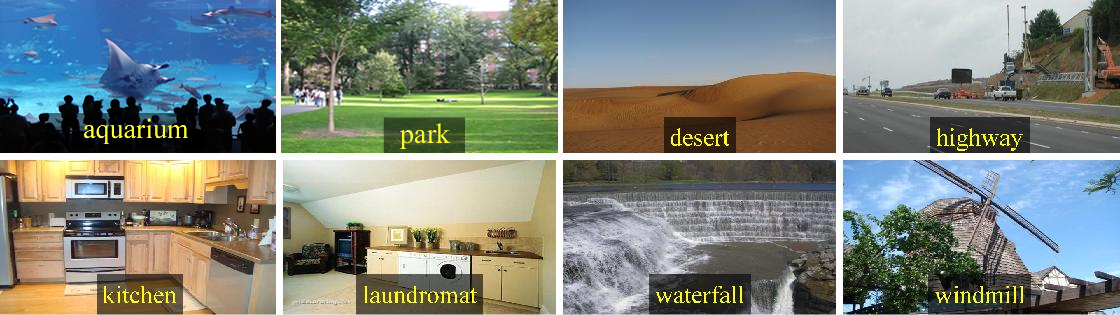
\includegraphics[width=\textwidth]{figures/teaser/teaser.png}
\caption{{\bf Scene Classification:} Given an image, can a computer program determine where it was taken? In this homework, you will build a representation based on bags of visual words and use spatial pyramid matching for classifying the scene categories.}
\label{fig:teaser}
\end{figure}


\section*{START HERE: Instructions}
\begin{itemize}
\item Please refer to the \href{https://canvas.cmu.edu/courses/32966/pages/logistics}{course logistics page} for information on the \textbf{Collaboration Policy} and \textbf{Late Submission Policy}.


\item\textbf{Submitting your work:} There will be two submission slots for this homework on \textbf{Gradescope}: Written and Programming. 

\begin{itemize}

\item 
For written problems such as short answer, multiple choice, derivations, proofs, or plots, we will be using the written submission slot. Please use this provided template. \textbf{We don't accept handwritten submissions.}  Each answer should be completed in the boxes provided below the question. You are allowed to adjust the size of these boxes, but \textbf{make sure to link your answer to each question when submitting to Gradescope}. Otherwise, your submission will not be graded.
\item
You are also required to upload your code, which you wrote to solve this homework, to the Programming submission slot. Your code may be run by TAs so please make sure it is in a workable state. The assignment must be completed using Python 3.7 or newer. We recommend setting up a \href{https://docs.conda.io/projects/conda/en/latest/user-guide/index.html}{conda environment}, but you are free to set up your environment however you like. 
\item
Regrade requests can be made after the homework grades are released, however this gives the TA the opportunity to regrade your entire paper, meaning if additional mistakes are found then points will be deducted. 
\end{itemize}

\item {\bf Start early!} This homework may take a long time to complete.

\item {\bf Attempt to verify your implementation as you proceed.} If you don't verify that your implementation is correct on toy examples, you will risk having a huge mess when you put everything together. Here are two tips:

(1) Once you write a function, uncomment the corresponding lines in \texttt{main.py} to verify whether the function executes correctly. 

(2) To debug your logic within a function, use \texttt{print()} or \texttt{breakpoint()}.
% (https://realpython.com/lessons/print-and-breakpoint/).  

\item Follow the guidelines in Section~\ref{sec:SubChecklist}: HW Checklist for writeup and code. If you have any questions or need clarifications, please post in Slack or visit the TAs during office hours. 

\end{itemize}

\clearpage

\section*{Overview}\label{sec:overview}

Bag-of-words (BoW) can be applied to many problems in computer vision, including object recognition~\cite{790410,1544935} and scene classification~\cite{renninger2004scene,5539970}\footnote{This homework is largely self-contained, but reading the listed papers (or even just skimming them) will likely be helpful.}. This homework will explore classic BoW along with extensions, such as pyramid matching~\cite{1544890,1641019} and feature encoding~\cite{Chatfield11}. Fig~\ref{fig:overview} provides an overview. Section~\ref{sec:visual_words} builds a dictionary of visual words from a training set of images by clustering. Section~\ref{sec:img_recog} builds a representation for a particular image as a histogram over visual words, or BoW. Finally, you will build a scene recognition system that classifies a test image by comparing it to a training library of images in BoW space (e.g., nearest-neighbor classification).
\begin{figure}[!h]
    \centering
    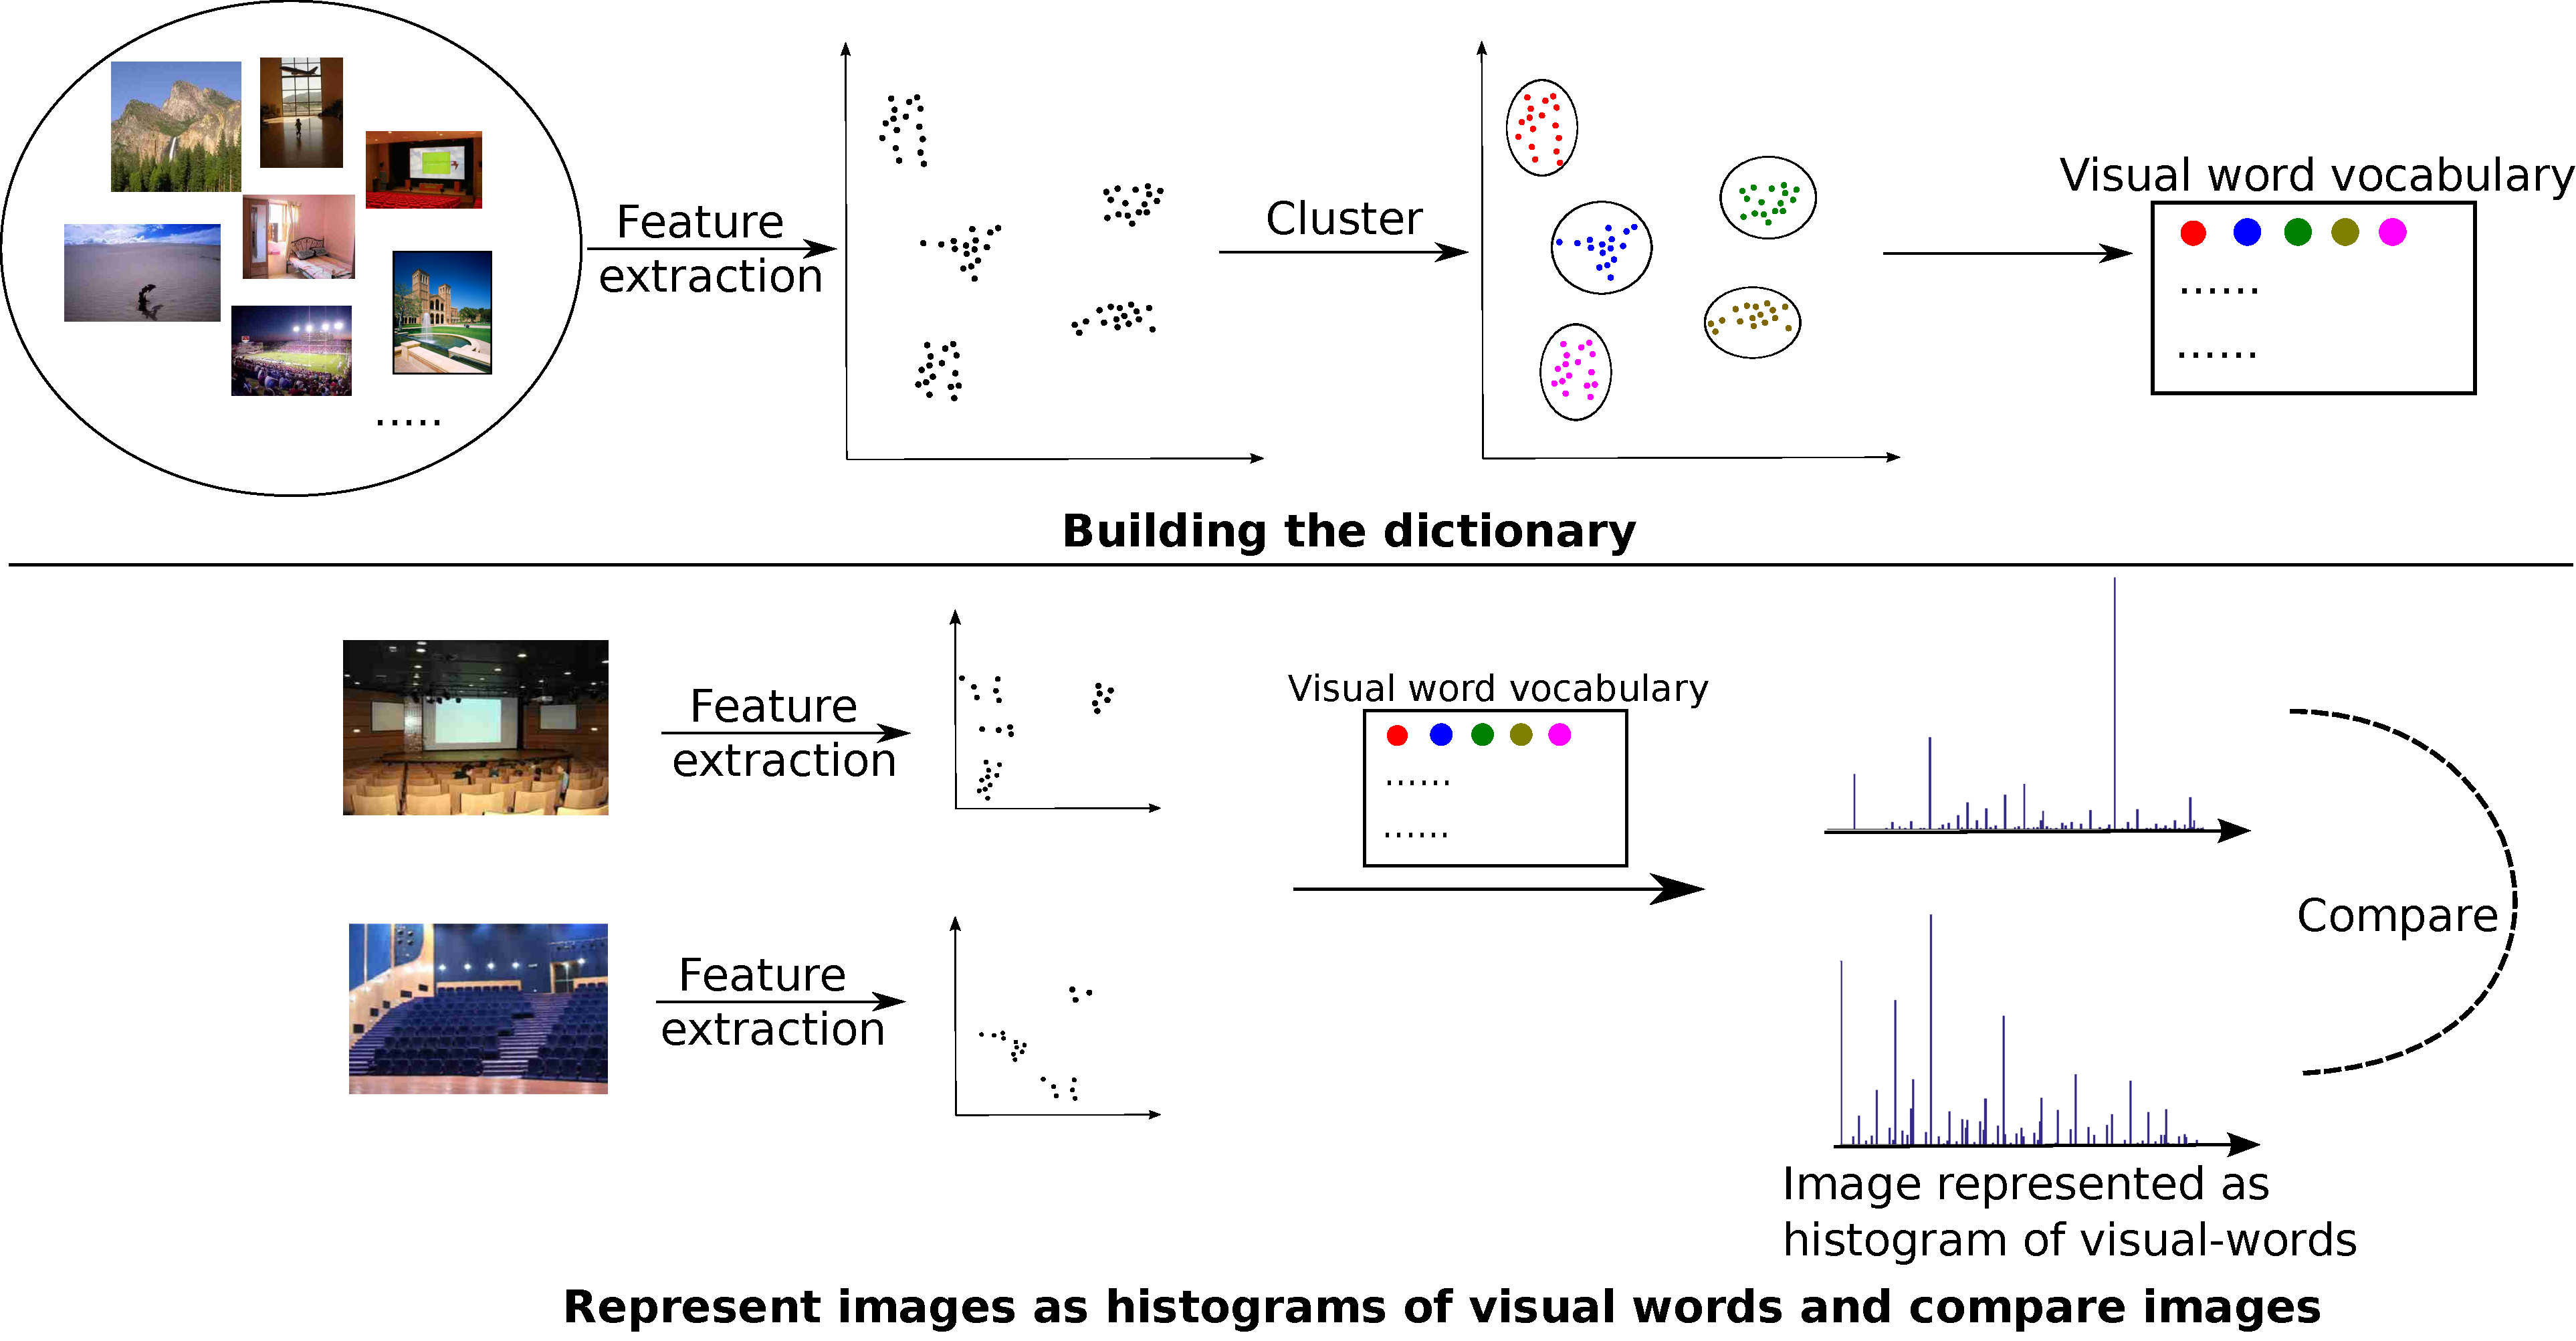
\includegraphics[width=\textwidth]{./figures/overview.pdf}
    \caption{An overview of the bags-of-words approach to be implemented in the homework. First, given the training set of images, we extract the visual features of the images. In our case, we will use the filter responses of the pre-defined filter bank as the visual features. Next, we build visual words, \ie a dictionary, by finding the centers of clusters of the visual features. To classify new images, we first represent each image as a vector of visual words, and then compare new images to old ones in the visual-word vector space -- the nearest match provides a label!}
    \label{fig:overview}
\end{figure}

\par \noindent {\bf What you will be doing:}
You will implement a scene classification system that uses the bag-of-words approach with its spatial pyramid extension. The paper that introduced the pyramid matching kernel~\cite{1544890} is
\begin{center}\parbox{5in}{
K. Grauman and T. Darrell. {\it The Pyramid Match Kernel: Discriminative Classification with Sets of Image Features}. ICCV 2005. \url{http://www.cs.utexas.edu/~grauman/papers/grauman_darrell_iccv2005.pdf}
}
\end{center}

Spatial pyramid matching~\cite{1641019} is presented in
\begin{center}\parbox{5in}{
S. Lazebnik, C. Schmid, and J. Ponce, {\it Beyond Bags of Features: Spatial Pyramid Matching for Recognizing Natural Scene Categories}, CVPR 2006. \url{http://www.di.ens.fr/willow/pdfs/cvpr06b.pdf}
}
\end{center}
You will be working with a subset of the SUN database\footnote{\url{http://groups.csail.mit.edu/vision/SUN/}}. The data set contains ~1600 images from various scene categories like ``aquarium, ``desert'' and ``kitchen''. And to build a recognition system, you will:
\begin{itemize}
	\item take responses of a filter bank on images and build a dictionary of visual words, and then  
	\item learn a model for images based on the bag of words (with spatial pyramid matching~\cite{1641019}), and use nearest-neighbor to predict scene classes in a test set.
\end{itemize}

In terms of number of lines of code, this assignment is fairly small. However, it may take {\it a few hours} to finish running the baseline system, so make sure you start early so that you have time to debug things. Try printing statements within long-running functions to verify that the function did not hang. Also, try {\bf each component} on {\bf a subset of the data set} first before putting everything together. We provide you with a number of functions and scripts in the hopes of alleviating some tedious or error-prone sections of the implementation. You can find a list of files provided in Section \ref{sec:Manifest}. {\em Though not necessary, you are recommended to implement a multi-processing\footnote{Note that multi-threading in python does not make use of multiple CPU cores. It may not work on windows jupyter notebook.} version to make use of multiple CPU cores to speed up the code}. Functions with {\tt n\_worker} as input can benefit greatly from parallel processing.

{\bf Hyperparameters:} We provide you with a basic set of hyperparameters, which might not be optimal. You will be asked in Q3.1 to tune the system you built and we suggest you to keep the defaults before you get to Q3.1. 
All hyperparameters can be found in a single configuration file {\tt opts.py}.

\clearpage

\section{Representing the World with Visual Words}
\label{sec:visual_words}

\begin{figure}
\centering
%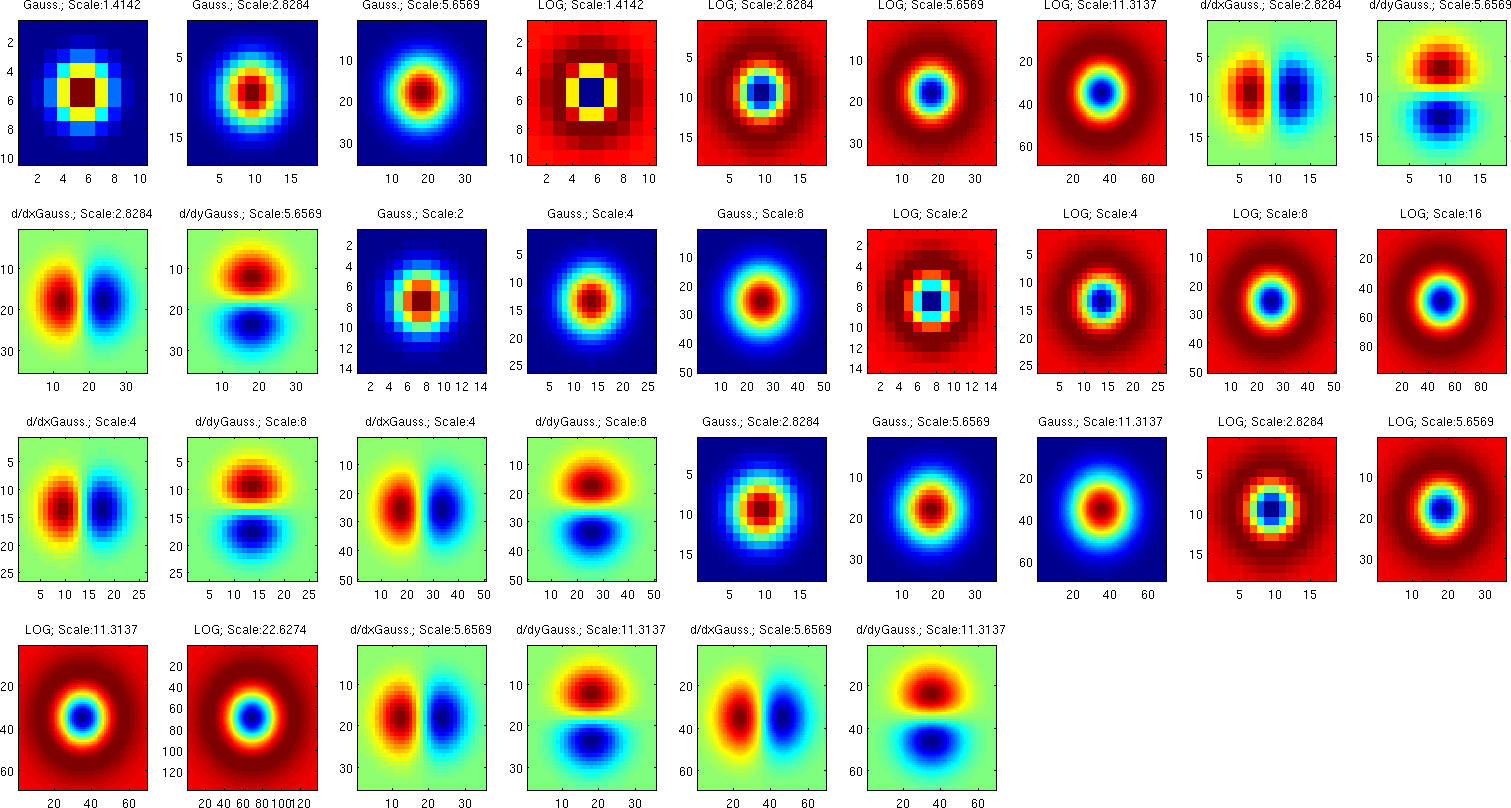
\includegraphics[width=0.9\textwidth]{figures/baselinefb.png}
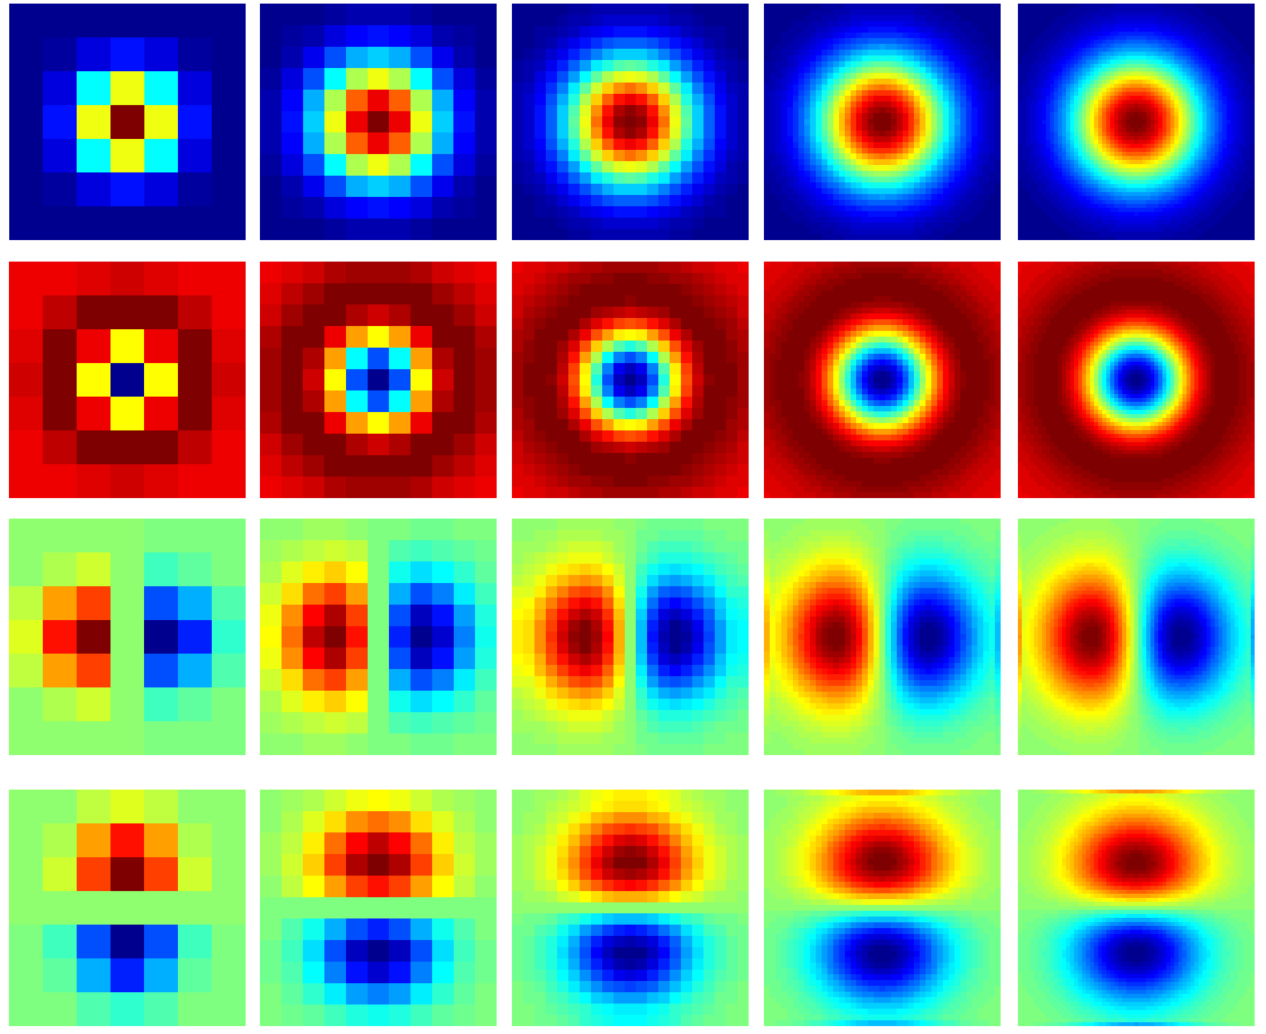
\includegraphics[width=.5\textwidth]{figures/filters.pdf}
\caption{Multi-scale filter bank}
\label{fig:fb}
\end{figure}

\begin{figure}[h]
  \centering
  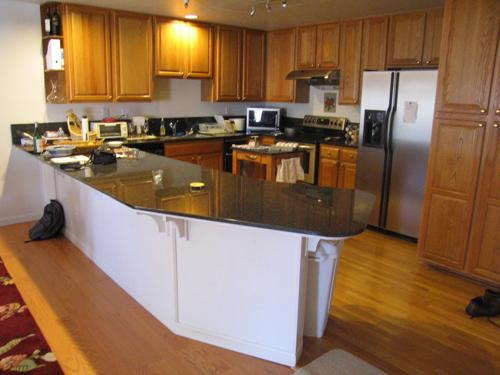
\includegraphics[width=.5\textwidth]{./figures/example_filter.jpg}
  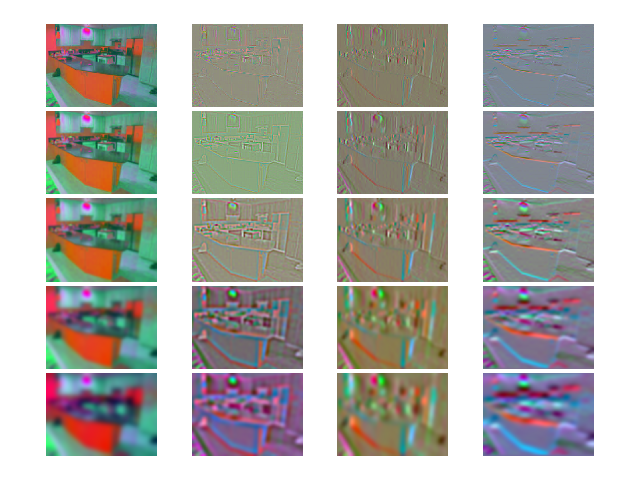
\includegraphics[width=.6\textwidth]{./figures/filters.png}
  \caption{An input image and filter responses for all of the filters in the filter bank. \textbf{Top:} The input image. 
    \textbf{Bottom:} The filter responses in Lab colorization, corresponding to the filters in Fig~\ref{fig:fb} (Transposed).}
  \label{fig:filter_resp}
\end{figure}

% We have provided you with a multi-scale filter bank that you will use to understand the visual world. You can create an instance of it with the following (provided) function:
% \begin{center}
%     {\tt [filterBank] = createFilterBank()}
% \end{center}

% {\tt filterBank} is a cell array\footnote{Look at MATLAB's documentation for more details, but {\tt filterBank\{i\}} is
% a 2D matrix, and {\tt filterBank\{i\}} and {\tt filterBank\{j\}} are not necessarily the same size.}, with the pre-defined filters
% in its entries. In our example, we are using $20$ filters consisting of $4$ types of filters in $5$ scales.\\

% \par \noindent {\bf Q1.0 (5 points):} What properties do each of the filter functions (See Fig~\ref{fig:fb}) pick up? You should group the filters into broad categories (\ie, all the Gaussians). Answer in your write-up.

\subsection{Extracting Filter Responses}

We want to run a filter bank on an image by convolving each filter in the bank with the image and concatenating all the responses into a vector for each pixel.
In our case, we will be using $4$ types of filters of multiple scales ({\tt opts.filter\_scales}).
The filters are: (1) Gaussian, (2) Laplacian of Gaussian, (3) derivative of Gaussian in the $x$ direction, and (4) derivative of Gaussian in the $y$ direction.
% The 5 scales we will be using are $1$, $2$, $4$, $8$, and $8\sqrt{2}$, in pixel units.
\par \noindent {\bf Q1.1.1 (5 points):}
(a) What properties do each of the filter functions pick up? (See Fig~\ref{fig:fb}) 
Try to group the filters into broad categories (\eg all the Gaussians). 

(b) Why do we need multiple scales of filter responses? 

\begin{your_solution}[title=Q1.1.1 (a)(b),height=6cm,width=\linewidth]
%solution 

\end{your_solution}

\par \noindent {\bf Q1.1.2 (10 points):} 
For the code, loop through the filters and the scales to extract responses. Since color images have $3$ channels, you are going to have a total of $3F$ filter responses per pixel if the filter bank is of size $F$. Note that in the given dataset, there are some gray-scale images. For those gray-scale images, you can simply duplicate them into three channels. Then output the result as a $3F$ channel image. Image $\texttt{laundromat/sun\_afrrjykuhhlwiwun.jpg}$ has 4 channels instead of 3. Discard the last channel. Try to first iterate across scales and then for each scale, iterate across each channel (i.e. Scale$_1$ \{Gaussian \{R,G,B\}, Laplacian \{R, G, B\}, ...\}, Scale$_2$ \{Gaussian\{R,G,B\}, Laplace\{R, G, B\}, ...\}). Use zero-padding if necessary. Normalize the input before passing the image to extract\_filter\_responses. Complete the function 
\begin{center}
    {\tt visual\_words.extract\_filter\_responses(opts, img)}
\end{center}
and return the responses as {\tt filter\_responses}.
We have provided you with template code, with detailed instructions commented inside. The convolution routine function {\tt scipy.ndimage.convolve()} can be used with user-defined filters, but the functions {\tt scipy.ndimage.gaussian\_filter()} and {\tt scipy.ndimage.gaussian\_laplace()} may be useful here for improved efficiency. Note that by default {\tt scipy.ndimage} applies filters to all dimensions including channels. Therefore you might want to filter each channel separately. You can also pass in a parameter indicating you want either the x or y derivative.

Remember to check the input argument {\tt image} to make sure it is a floating point type with range $[0, 1]$, and convert it if necessary. Be sure to check the number of input image channels and convert it to 3-channel if it is not. Before applying the filters, use the function {\tt skimage.color.rgb2lab()} to convert your image into the {\tt Lab} color space, which is designed to more effectively quantify color differences with respect to human perception. (See {\bf \href{https://en.wikipedia.org/wiki/CIELAB_color_space}{here}} for more information.) If the input {\tt image} is an $M \times N \times 3$ matrix, then {\tt filter\_responses} should be a matrix of size $M \times N \times 3F$. Make sure your convolution function call handles image padding along the edges sensibly.

Apply all 4 filters at least 3 scales on {\tt aquarium/sun\_aztvjgubyrgvirup.jpg}, and visualize the responses as an image collage as shown in Fig~\ref{fig:filter_resp}. To plot the collage, you can use the included helper function {\tt util.display\_filter\_responses} by providing a list of filter responses with those of the Lab channels grouped together with shape $M \times N \times 3$. We provide the skeleton code from line 17-21 in {\tt main.py}. You can get the results by running {\tt python main.py --filter-scales 1 2 4}.


% {\bf Submit the collage of images in your write-up.}

\begin{your_solution}[title=Q1.1.2,height=17cm,width=\linewidth]
%solution 

\end{your_solution}

\subsection{Creating Visual Words}
You will now create a dictionary of visual words from the filter responses using k-means. After applying k-means, similar filter responses will be represented by the same visual word. You will use a dictionary with a fixed size. Instead of using all of the filter responses ({\bf which might exceed the memory capacity of your computer}), you will use responses at $\alpha$ random pixels. If there are $T$ training images, then you should collect a matrix {\tt filter\_responses} over all the images that is $\alpha T \times 3F$, where $F$ is the filter bank size.
Then, to generate a visual words dictionary with $K$ words ({\tt opts.K}), you will cluster the responses with k-means using the function {\tt sklearn.cluster.KMeans} as follows:
\begin{center}
    {\tt kmeans = sklearn.cluster.KMeans(n\_clusters=K).fit(filter\_responses) \\
    dictionary = kmeans.cluster\_centers\_ }
\end{center}
If you like, you can pass the {\tt n\_jobs} argument into the {\tt KMeans()} object to utilize parallel computation. \\

% Note that the output of the function {\tt kmeans} is row-wise, \ie, each row is an sample/cluster.
% In our following implementations, we will assume the dictionary matrix is column-wise. So you need to transpose {\tt dictionary}
% after it is estimated from the {\tt kmeans} function.\\

\par \noindent {\bf Q1.2 (10 points):}
Write the functions
\begin{center}
  {\tt visual\_words.compute\_dictionary(opts, n\_worker)}, \\
  {\tt visual\_words.compute\_dictionary\_one\_image(args)} (optional, multi-processing),
\end{center}
Given a dataset, these functions generate a dictionary. 
The overall goal of {\tt compute\_dictionary()} is to load the training data, iterate through the paths to the image files to read the images, and extract $\alpha T$ filter responses over the training files, and call k-means.
This can be slow to run; however, the images can be processed independently and in parallel.
Inside {\tt compute\_dictionary\_one\_image()}, you should read an image, extract the responses, and save to a temporary file. Here {\tt args} is a collection of arguments passed into the function.
Inside {\tt compute\_dictionary()}, you should load all the training data and create subprocesses to call {\tt compute\_dictionary\_one\_image()}.
After all the subprocesses finish, load the temporary files back, collect the filter responses, and run k-means. A list of training images can be found in {\tt data/train\_files.txt}.

Finally, execute {\tt compute\_dictionary()}, and go do some push-ups while you wait for it to complete. 
If all goes well, you will have a file named {\tt dictionary.npy} (with size of $K \times 3F$) that contains the dictionary of visual words. 
If the clustering takes too long, reduce the number of clusters and samples. You can start with a tiny subset of training images for debugging. We provide the skeleton code from line 24-25 in {\tt main.py}. You can get the results by running {\tt python main.py --filter-scales 1 2 4 --feat-dir TMP\_OUT\_DIR\_FOR\_EACH\_IMG --out-dir FINAL\_OUT\_DIR}.


\textbf{Include your implemented functions  within the \texttt{minted} block below} 
{\tt compute\_dictionary}, and optionally, {\tt compute\_dictionary\_one\_image} or other customized functions).
% . You can simply include a screenshot or copy/paste it into a {\tt verbatim} / {\tt lstlisting} environment.

\begin{your_solution}[title=Q1.2,height=23 cm,width=\linewidth]
%solution 
\begin{minted}
[
framesep=2mm,
baselinestretch=1.2,
fontsize=\footnotesize,
% linenos, 
breaklines
]
{python}
# Copy and paste your code here.
\end{minted}

\end{your_solution}

\subsection{Computing Visual Words}

\begin{figure}[h]
  \centering
  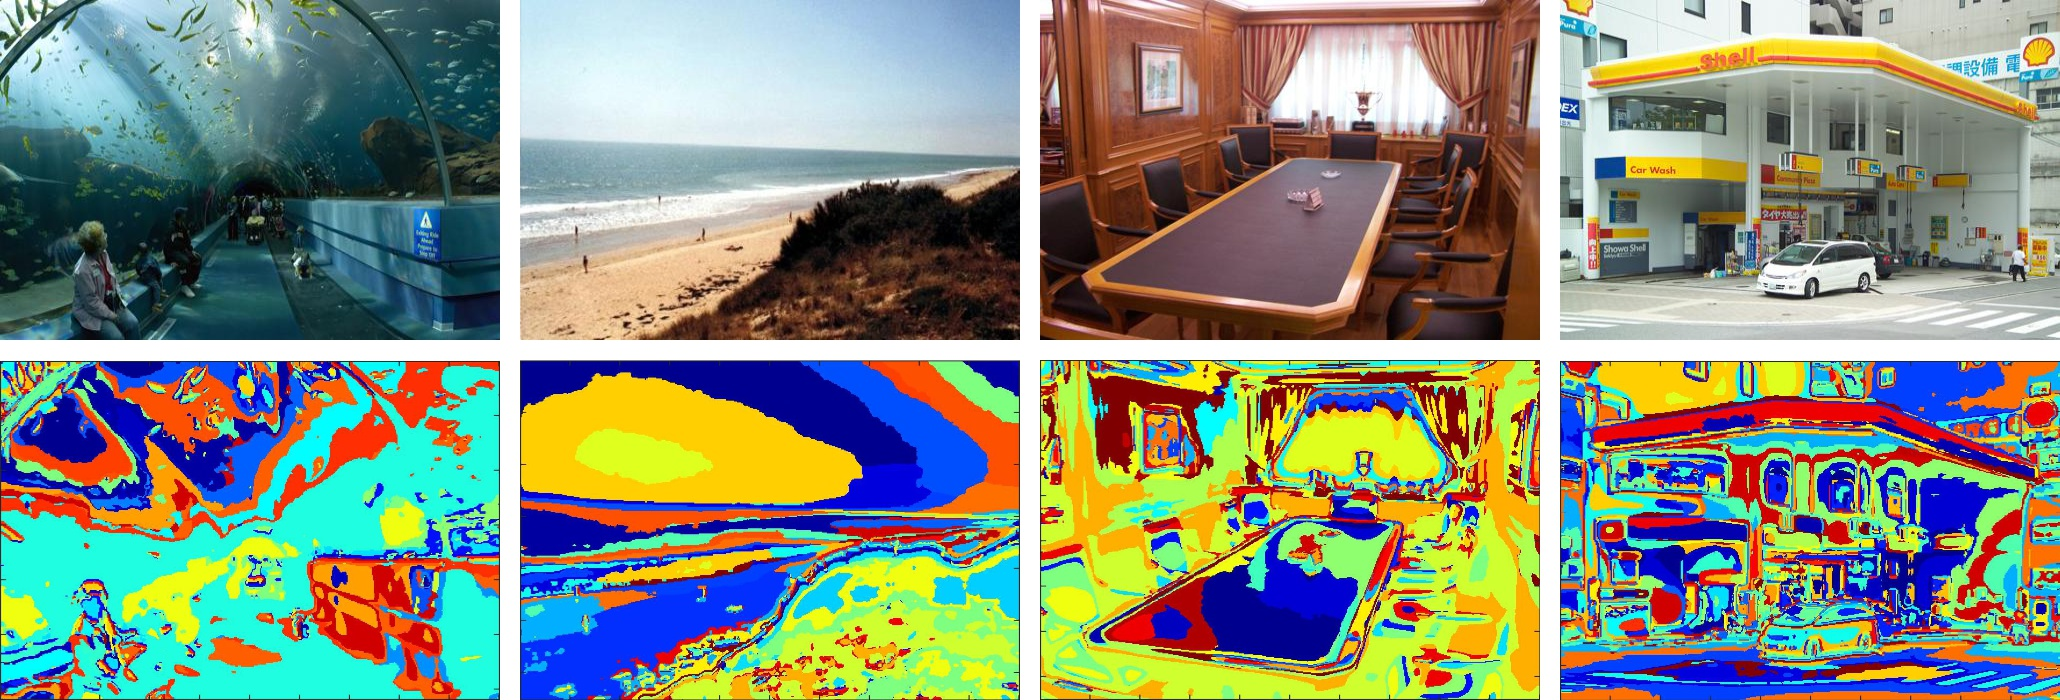
\includegraphics[width=\textwidth]{./figures/textons.jpg}
  \caption{Visual words over images. You will use the spatially unordered
    distribution of visual words in a region (a bag of visual words) as a
    feature for scene classification, with some coarse information provided by
    spatial pyramid matching~\cite{1641019}.}
  \label{fig:textons}
\end{figure}

{\bf Q1.3 (10 points):}
We want to map each pixel in the image to its closest word in the dictionary.
Complete the following function to do this:
\begin{center}
{\tt visual\_words.get\_visual\_words(opts, img, dictionary)}
\end{center}
and return {\tt wordmap}, a matrix with the same width and height as {\tt img}, where each pixel in {\tt wordmap} is assigned the closest visual word of the filter response at the respective pixel in {\tt img}. We will use the standard Euclidean distance to do this; to do this efficiently, use the function {\tt scipy.spatial.distance.cdist()}. Some sample results are shown in Fig~\ref{fig:textons}.

% Since this can be slow, we have provided a function {\tt batchToVisualWords(numberOfCores)} that will apply your implementation of the function {\tt getVisualWords} to every image in the training and testing set. This function will automatically\footnote{Interested parties should investigate {\tt batchToVisualWords.m} and the MATLAB commands {\tt matlabpool} and {\tt parfor}.} use as many cores as you tell it to use. For every image ``{\tt X.jpg}'' in {\tt dat/}, there will be a corresponding file named ``{\tt X.mat}'' in the same folder containing the variable {\tt wordMap}.

{\bf Visualize wordmaps for three images. Include some comments on these visualizations: do the ``word'' boundaries make sense to you?} The visualizations should look similar to the ones in Fig~\ref{fig:textons}. Don't worry if the colors don't look the same, newer {\tt matplotlib} might use a different color map.

We provide the skeleton code from line 28-33 in {\tt main.py}. You can get the results by running {\tt python main.py --filter-scales 1 2 4 --feat-dir TMP\_OUT\_DIR\_FOR\_EACH\_IMG --out-dir FINAL\_OUT\_DIR}.

\begin{your_solution}[title=Q1.3,height=23cm,width=\linewidth]
%solution 

\end{your_solution}

\clearpage


\section{Building a Recognition System}
\label{sec:img_recog}
We have formed a convenient representation for recognition. We will now
produce a basic recognition system with spatial pyramid matching. The goal of the system is presented in Fig~\ref{fig:teaser}:
given an image, classify (i.e., recognize/name) the scene depicted in the image.

Traditional classification problems follow two phases: training and testing.
At training time, the computer is given a pile of formatted data (\ie, a collection
of feature vectors) with corresponding labels (\eg, ``desert'', ``park'') and
then builds a model of how the data relates to the labels (\eg, ``if green, then park''). At test time, the computer takes features and uses these rules to infer the label (\eg, ``this is green, therefore it is a park'').

In this assignment, we will use the simplest classification method: nearest neighbor.
At test time, we will simply look at the query's nearest neighbor in the training set
and transfer that label. In this example, you will be looking
at the query image and looking up its nearest neighbor in a collection of training images whose labels are already known. This approach works
surprisingly well given a huge amount of data. (For a cool application, see the work by Hays \& Efros~\cite{Hays:2007}). 

The key components of any nearest-neighbor system are:
\begin{itemize}
\item features (how do you represent your instances?) and
\item similarity (how do you compare instances in the feature space?).
\end{itemize} You will implement both.

\subsection{Extracting Features}

We will first represent an image with a bag of words. In each image, we simply look at how often each word appears.
\par ~
\par \noindent {\bf Q2.1 (10 points):}
Write the function
\begin{center}
{\tt visual\_recog.get\_feature\_from\_wordmap(opts, wordmap)}
\end{center}
that extracts the histogram ({\tt numpy.histogram()}) of visual words within the given image
(\ie, the bag of visual words).
% As inputs, the function will take:
% \begin{itemize}
% \setlength{\parskip}{0pt}
% \item {\tt wordmap}, a {\tt H} $\times$ {\tt W} image containing the IDs of the visual words
% \item {\tt dict\_size}, the maximum visual word ID (\ie, the number of visual words, the dictionary size). Notice that your histogram should have {\tt dict\_size} different bins.
% \end{itemize}
As output, the function will return {\tt hist}, an
``$L_1$ normalized'' {\tt dict\_size}-length histogram The $L_1$ normalization makes the sum of the histogram equal to $1$. 
You may wish to load a single visual word map, visualize it, and verify that your function is working correctly before proceeding.

% \textbf{Please submit your code following the guidelines in Section~\ref{sec:SubChecklist}.}
\textbf{Include your implemented functions  within the \texttt{minted} block below}.
% . You can simply include a screenshot or copy/paste it into a {\tt verbatim} / {\tt lstlisting} environment.

\begin{your_solution}[title=Q2.1,height=23 cm,width=\linewidth]
%solution 
\begin{minted}
[
framesep=2mm,
baselinestretch=1.2,
fontsize=\footnotesize,
% linenos, 
breaklines
]
{python}
# Copy and paste your code here.
\end{minted}

\end{your_solution}


\subsection{Multi-resolution: Spatial Pyramid Matching}
A bag of words is simple and efficient, but it discards information about the spatial structure of the image and this information is often valuable. 
One way to alleviate this issue is to use spatial pyramid matching~\cite{1641019}. The general idea is to divide the image into a small number of cells, and concatenate the histogram of each of these cells to the histogram of the original image, with a suitable weight. 

Here we will implement a popular scheme that chops the image into $2^l\times2^l$ cells where $l$ is the layer number. We treat each cell as a small image and count how often each visual word appears. This results in a histogram for every single cell in every layer. Finally to represent the entire image, we concatenate all the histograms together after normalization by the total number of features in the image. If there are $L+1$ layers and $K$ visual words, the resulting vector has dimension $K\sum_{l=0}^L{4^l} = K\left(4^{(L+1)}-1\right)/3$.

Now comes the weighting scheme. Note that when concatenating all the histograms, histograms from different levels are assigned different weights. Typically (and in the original work~\cite{1641019}), a histogram from layer $l$ gets half the weight of a histogram from layer $l+1$, with the exception of layer 0, which is assigned a weight equal to layer 1. A popular choice is to set the weight of layers $0$ and $1$ to $2^{-L}$, and set the rest of the weights to $2^{l-L-1}$ (\eg, in a three layer spatial pyramid, $L=2$ and weights are set to $1/4$, $1/4$ and $1/2$ for layer 0, 1 and 2 respectively. See Fig~\ref{fig:spm} for an illustration of a spatial pyramid. Note that the $L_1$ norm (absolute values of all dimensions summed up together) for the final vector is 1.

\begin{figure}[h]
\centering
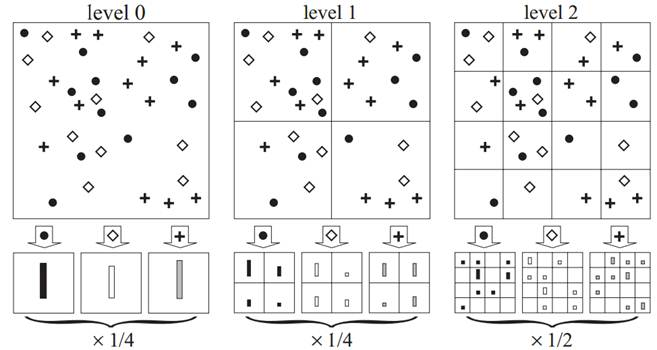
\includegraphics[width=0.6\textwidth]{figures/spm.jpg}
\caption{{\bf Spatial Pyramid Matching:} From \cite{1641019}. Toy example of a pyramid for L = 2. The image has three visual words, indicated by circles, diamonds, and crosses. We subdivide
the image at three different levels of resolution. For each level of resolution
and each channel, we count the features that fall in each spatial bin. Finally, 
weight each spatial histogram.}
\label{fig:spm}
\end{figure}

\par \noindent {\bf Q2.2 (15 points):}
Create a function {\tt get\_feature\_from\_wordmap\_SPM} that forms a multi-resolution representation of the given image.

\begin{center}
{\tt visual\_recog.get\_feature\_from\_wordmap\_SPM(opts, wordmap)}
\end{center}
You need to specify the layers of pyramid in {\tt opts.L} (Note there are $L+1$ layers in total). 
% As inputs, the function will take:
% \begin{itemize}
% \setlength{\parskip}{0pt}
% \item {\tt layer\_num}, the number of layers in the spatial pyramid, \ie, $L+1$
% \item {\tt wordmap}, a {\tt H} $\times$ {\tt W} image containing the IDs of the visual words
% \item {\tt dict\_size}, the maximum visual word ID (\ie, the number of visual words / the dictionary size)
% \end{itemize}
As output, the function will return {\tt hist\_all}, a vector that is $L_1$ normalized. 
% {\bf Use a 3-layer spatial pyramid ($L=2$) for all of the following recognition tasks.}

One small hint for efficiency: a lot of computation can be saved if you first compute the histograms of the {\it finest} layer, because the histograms of coarser layers can then be aggregated from finer ones. Make sure you normalize the histogram after aggregation.

\textbf{Include your implemented functions  within the \texttt{minted} block below}.

\begin{your_solution}[title=Q2.2,height=23 cm,width=\linewidth]
%solution 
\begin{minted}
[
framesep=2mm,
baselinestretch=1.2,
fontsize=\footnotesize,
% linenos, 
breaklines
]
{python}
# Copy and paste your code here.
\end{minted}

\end{your_solution}


\subsection{Comparing images}

We need a way to compare images, to find the ``nearest'' instance in the training data.
In this assignment, we'll use the histogram intersection similarity. The histogram
intersection similarity between two histograms is the sum of the minimum value of each corresponding bins.
% $h_1$ and $y_{1:n}$ is defined as $\sum_{i=1}^n \min(x_i,y_i)$, or
% {\tt sum(min(x,y))} in MATLAB.
This is a similarity score: the {\it largest} value indicates the ``nearest'' instance.
\par ~
\par \noindent {\bf Q2.3 (10 points):}
Create the function
\begin{center}
{\tt visual\_recog.distance\_to\_set(word\_hist, histograms)}
\end{center}
where {\tt word\_hist} is a $K\left(4^{(L+1)}-1\right)/3$ vector
and {\tt histograms} is a $T \times K\left(4^{(L+1)}-1\right)/3$ matrix containing $T$ features
from $T$ training samples concatenated along the rows. This function
computes the histogram intersection similarity between {\tt word\_hist}
and each training sample as a vector of length $T$ and returns one minus the above quantity as a distance measure (distance is the inverse of similarity).
Since this is called every time you look up a classification, you will want this to be fast! (Doing a for-loop over tens of thousands of histograms is a bad idea.) Note: $\texttt{laundromat/sun\_afrrjykuhhlwiwun.jpg}$ has 4 channels instead of 3. Discard the last channel.
% Try {\tt repmat} or (even faster) {\tt bsxfun}\footnote{As a recommendation: unless you're experienced with MATLAB or confident, make sure your optimization works before moving on. Either use a few hand-made examples that you can manually verify  or subtract the distances produced by the unoptimized and optimized examples.}.

\textbf{Include your implemented functions  within the \texttt{minted} block below}.

\begin{your_solution}[title=Q2.3,height=23 cm,width=\linewidth]
%solution 
\begin{minted}
[
framesep=2mm,
baselinestretch=1.2,
fontsize=\footnotesize,
% linenos, 
breaklines
]
{python}
# Copy and paste your code here.
\end{minted}

\end{your_solution}

\subsection{Building A Model of the Visual World}

Now that we've obtained a representation for each image, and defined a similarity measure to compare two spatial pyramids, we want to put everything up to now together.

Simple I/O code has been provided in the respective functions, which include loading the training images specified in {\tt data/train\_files.txt} and the filter bank and visual word dictionary from {\tt dictionary.npy}, and also saving the learned model to {\tt trained\_system.npz}. Specifically in {\tt trained\_system.npz}, you should have:
\begin{enumerate}
\setlength{\parskip}{0pt}
\item {\tt dictionary}: your visual word dictionary.
\item {\tt features}: an $N \times  K\left(4^{(L+1)}-1\right)/3$ matrix containing all of
the histograms of the $N$ training images in the data set.
\item {\tt labels}: an $N$ vector containing the labels
of each of training images. ({\tt features[i]} will correspond to label {\tt labels[i]}).
\item {\tt SPM\_layer\_num}: the number of spatial pyramid layers you used to extract the features for the training images.
\end{enumerate}

{\bf Do not use the testing images for training!}\\

The table below lists the class names that correspond to the label indices:
% You may also wish to convert the labels to meaningful categories. Here is the mapping (a variable named {\tt mapping} is included in {\tt traintest.mat}):\\
\begin{center}
\begin{tabular}{c@{~~}c@{~~}c@{~~}c@{~~}c@{~~}c@{~~}c@{~~}c} \toprule
0 & 1 & 2 & 3 & 4 & 5 & 6 & 7 \\ \midrule
aquarium & desert & highway & kitchen & laundromat & park & waterfall & windmill\\ \bottomrule
%abbey & airport & bamboo\_forest & bar & bus\_shelter & canyon & computer\_room \\ \midrule
%8 & 9 & 10 & 11 & 12 & 13 & \\ \midrule
%desert & dirt\_track & farm & fountain & glacier & highway & \\ \midrule
%14 & 15 & 16 & 17 & 18 & 19 & 20 \\ \midrule
%jail\_cell & kitchen & mountain & nightclub & ocean & restroom & sky \\ \midrule
%21 & 22 & 23 & 24 & 25 & 26 & \\ \midrule
%street & train\_railway & utility\_room & volcano & waterfall & zoo & \\ \bottomrule
\end{tabular} \\
\end{center}

\par \noindent
{\bf Q2.4 (15 points):}
Implement the function
\begin{center}
{\tt visual\_recog.build\_recognition\_system()} 
\end{center}
that produces {\tt trained\_system.npz}. You may include any helper functions you write in {\tt visual\_recog.py}.

Implement 
\begin{center}
{\tt visual\_recog.get\_image\_feature(opts, img\_path, dictionary)} 
\end{center}
that loads an image, extract word map from the image, computes the SPM, and returns the computed feature. Use this function in your {\tt visual\_recog.build\_recognition\_system()}.

We provide the skeleton code from line 36-37 in {\tt main.py}. You can train the model by running {\tt python main.py --filter-scales 1 2 4 --feat-dir TMP\_OUT\_DIR\_FOR\_EACH\_IMG --out-dir FINAL\_OUT\_DIR}.

\textbf{Include your implemented functions  within the \texttt{minted} block below}.

\begin{your_solution}[title=Q2.4,height=23 cm,width=\linewidth]
%solution 
\begin{minted}
[
framesep=2mm,
baselinestretch=1.2,
fontsize=\footnotesize,
% linenos, 
breaklines
]
{python}
# Copy and paste your code here.
\end{minted}

\end{your_solution}
% To qualitatively evaluate what you have done, we have provided a helper function {\tt } that will let you get the predictions on a new image given the training data. This will give you a visual sanity check that you have implemented things correctly. Use the program as follows:

% \begin{center}
% {\tt guessImage(absolutePathToImage)}%,~~~~~~~~~~(\eg, {\tt guessImage('more/CMU-1.jpg')})
% \end{center}

% The program will load the image, represent it with visual words,
% and get a prediction based on the histogram. The predictions will appear
% inside your MATLAB command window as text.

% Don't worry if you get a fair amount of wrong answers. Do worry if the program crashes
% while calling your code or if you get zero correct/all correct/all same answers. If you are getting
% 0\% or 100\% performance, go back and verify (visually) that each of your components produces correct output, or check that testing data are accidentally included during training (yet you can pick images from both training and testing set for debugging purposes).

\subsection{Quantitative Evaluation}

Qualitative evaluation is all well and good (and very important
for diagnosing performance gains and losses), but we want some hard numbers.

Load the test images and their labels, and compute the predicted
label of each one. That is, compute the test image's distance to every image in the training set, and return the label of the closest training image. To quantify the accuracy, compute a confusion matrix {\tt C}. In a classification problem, the entry {\tt C(i,j)} of a confusion matrix counts the number of instances of class {\tt i} that were predicted as class {\tt j}. When things are going well, the elements on the diagonal of {\tt C} are large, and the off-diagonal elements are small. Since there are 8 classes, {\tt C} will be $8 \times 8$. The accuracy, or percent of correctly classified images, is given by the trace of {\tt C} divided by the sum of {\tt C}. \textbf{Hint:} The accuracy with default parameters is ~50\%.
 \\

\par \noindent {\bf Q2.5 (10 points):}
Implement the function
\begin{center}
{\tt visual\_recog.evaluate\_recognition\_system()} 
\end{center}
that tests the system and outputs the confusion matrix.
{\bf Report the (a) confusion matrix and your (b) overall accuracy.} This does not have to be formatted prettily: \eg, you can simply copy/paste it into a {\tt verbatim} environment. 
% Additionally, do not worry if your accuracy is low: with 8 classes, chance is $12.5\%$.

\begin{your_solution}[title=Q2.5 (a) (b), height=10cm]
\end{your_solution}

\subsection{Find the failures}
There are some classes/samples that are more difficult to classify than the rest using the bags-of-words approach. As a result, they are classified incorrectly into other categories.\\

\par \noindent {\bf Q2.6 (5 points):}
Include some images of these hard classes/samples, and discuss why they are more difficult than the rest. 

\begin{your_solution}[title=Q2.6, height=21cm]
\end{your_solution}

\clearpage

\section{Improving performance}

\subsection{Hyperparameter tuning}

Now we have a full-fledged recognition system plus an evaluation system, it's time to boost up the performance. In practice, it is most likely that a model will not work well out-of-the-box. It is important to know how to tune a visual recognition system for the task at hand. \\

\par \noindent {\bf Q3.1 (15 points):} Tune the system you build to reach around 65\% accuracy on the provided test set ({\tt data/test\_files.txt}). A list of hyperparameters you should tune is provided below. They can all be found in {\tt opts.py}.
\begin{itemize}
    \item {\tt filter\_scales}: a list of filter scales used in extracting filter response;
    \item {\tt K}: the number of visual words and also the size of the dictionary;
    \item {\tt alpha}: the number of sampled pixels in each image when creating the dictionary;
    \item {\tt L}: the number of spatial pyramid layers used in feature extraction.
\end{itemize}
 (a) Include a table of ablation study containing at least 3 major steps (changing parameter X to Y achieves accuracy Z\%). 
 (b) Also, describe why you think changing a particular parameter should increase or decrease the overall performance in the table you show.



\begin{your_solution}[title=Q3.1 (a) (b), height=12cm]
\end{your_solution}


\subsection{[Extra Credit] Further improvement}
 \par \noindent {\bf Q3.2 (10 points):} Can you improve your classifier, in terms of accuracy or speed? Be creative! Or be well-informed, and cite your sources! For some quick ideas, try resizing the images, subtracting the mean color, changing the structure or weights of the spatial pyramid, or replacing the histogram intersection with some other similarity score. Whatever you do, explain:

(1) what you did,
 
(2) what you expected would happen, and 

(3) what actually happened. 

Include these results in the report and submit the code.

\begin{your_solution}[title=Q3.2, height=16cm]
\end{your_solution}

\clearpage

\section{HW1 Distribution Checklist}
\label{sec:Manifest}
After unpacking {\tt hw1.zip}, you should have a folder {\tt hw1} containing
one folder for the data ({\tt data}), one for your code ({\tt code}), and one for the report ({\tt latex}).
In the {\tt code} folder, where you will primarily work, you will find:
\begin{itemize}
\item {\tt visual\_words.py}: function definitions for extracting visual words.
\item {\tt visual\_recog.py}: function definitions for building a visual recognition system.
% \item {\tt network\_layers.py}: function definitions for implementing deep network layers.
\item {\tt util.py}: some utility functions
\item {\tt main.py}: main function for running the system

\end{itemize}

% Apart from this, we have also provided the stub codes in {\tt matlab} folder.
The data folder contains:

\begin{itemize}
\item {\tt data/}: a directory containing {\tt .jpg} images from the SUN database.
%\item {\tt data/more/}: a dataset containing some images that are collected from Google for qualitative evaluation.
\item {\tt data/train\_files.txt}: a text file containing a list of training images.
\item {\tt data/train\_labels.txt}: a text file containing a list of training labels.
\item {\tt data/test\_files.txt}: a text file containing a list of testing images.
\item {\tt data/test\_labels.txt}: a text file containing a list of testing labels.

% \item {\tt data/train\_data.npz}: a {\tt .npz} file containing the training set.
% \item {\tt data/test\_data.npz}: a {\tt .npz} file containing the test set.
% \item {\tt data/vgg16\_list.npy}: a {\tt .npy} file with the weights of VGG-16.

% \item {\tt checkA1Submission.m} Script to verify that your submission ($<$AndrewId$>$.zip) is in correct structure and contains all required files for submission.
\end{itemize}

\section{HW1 submission checklist}
\label{sec:SubChecklist}
Submit your write-up and code to Gradescope.
\begin{itemize}
\item {\bf Writeup.} Please use this provided template for your writeup.
  The write-up should be a pdf file named {\bf $<$AndrewId$>$\_hw1.pdf}. \textbf{You must select the pages of the writeup that correspond to each question}. 
  % Your writeup should include your answers to the following:
  % \begin{itemize}
  % \item Q1.1.1 (around 4 lines of text)
  % \item Q1.1.2 (visualization of filter responses)
  % \item Q1.3 (visualization of wordmaps)
  % \item Q2.5 (a confusion matrix, and an accuracy value)
  % \item Q2.6 (hard examples, and an explanation)
  % \item Q3.1 (table of ablation study and your final accuracy)
  % \item (Extra Credit) Q3.2 (model improvements)
  % \end{itemize}
\item {\bf Code.} 
The code should be submitted as a zip file named {\bf $<$AndrewId$>$\_hw1.zip}. By extracting the zip file, it should have the following files in the structure defined below.

{\bf When you submit, remove the folder {\tt data/} and {\tt feat/} if applicable, as well as any large temporary files that we did not ask you to create.}

\begin{itemize}
\item {\bf $<$andrew\_id$>$/ }  \# A directory inside .zip file
\begin{itemize}
	\item {\tt code/ }
	\begin{itemize}
		\item {\tt dictionary.npy }
		\item {\tt trained\_system.npz }
		\item $<$!-- all of your .py files $>$
	\end{itemize}
    \item {\tt $<$andrew\_id$>$\_hw1.pdf}  make sure you upload this pdf file to Gradescope. Please assign the locations of answers to each question on Gradescope.
\end{itemize}

\end{itemize}
\end{itemize}

\bibliographystyle{plain}
\bibliography{refs}

\end{document}

